\section{Introduction}

Knowledge Graph (KG) has been deployed in a large amount of enterprises nowadays. In e-commerce scenario, KGs can benefit a lot of downstream tasks, such as Product Search Relevance (PSR), recommendation, Question Answering (QA) etc. In this paper, we focus on utilizing KG to improve PSR task in e-commerce. 

\xiujie{With the development of e-commerce, a new e-commerce mode called life service e-commerce is emerging, which is a kind of Online-To-Offline (O2O) e-commerce. Life service e-commerce allows users to order almost all the products from offline shops near them in their city online through their mobile-phone, which means the range of these products covers almost all the types of products we can see in our daily life, including fruits, vegetables, medicine, flowers, etc. } Though life service e-commerce is convenient for users, huge variety of products also makes PSR task more challenging. 
One of the most challenging problem in such scenario is that we may not know what a product exactly is with only product name as they may have various synonyms. The reason behind this problem is that these products are too close to people's daily life, so that different people or people from different regions may have different names for the same product. 
Besides, in order to make the product name more attractive, some product names are also designed to be more vivid and interesting, which makes it more difficult to understand the product. For example, ``Seaweed-flavored shallots green onion 65g'' is a kind of snack, but it is hard to tell what it is with only its name. 
All these challenges make external knowledge necessary for this task and KG can be a good option. 

% Furthermore, typos also add difficulty to this task. 

% In such scenario, product category covers almost all products we can see in all markets and shops in one city, including all kinds of fruits, vegetables, snacks etc.
% Online takeaway is one of the most typical examples of life service e-commerce.
% \sansa{Emphasizing Chinese narrows the scope of motivation}
% \zelin{suggestion: ... are comprehensively understood by the model}
% \zelin{the world?}
%  which means KG can help model understand objective things better
The core idea of fusing KG into PSR model is that with the help of KG, the intent of user query and the product referred to by the product name can be clarified with their relations with concepts or products in KG. 
That is because products are usually linked on concepts in the taxonomy and user queries themselves are sometimes concepts in KG. 
Thus, knowledge related to queries and products can be retrieved from KG.

The overview of PSR task with KG in e-commerce is depicted in Figure \ref{fig:taskoverview}. 
Generally speaking, there is usually a hierarchical taxonomy formed via isA relations to organize products and concepts in e-commerce KG. 
This taxonomy is usually manually defined and coarse-grained. The concepts are usually product categories and organized in the higher levels of taxonomy, for example, ``Vegetables / Rhizomes / Potatoes'' is a three-level path consisting of three concepts in taxonomy. 
Products are usually linked on the most fine-grained concepts as leaf nodes of the taxonomy. 
For instance, the product ``5 fresh potatoes'' is linked on the path.
To better understand user needs and product names, a more fine-grained e-commerce related concept graph is usually constructed and these concepts are connected via other types of relations, such as \textit{synonym} and \textit{related\_to}.
These relations are defined to further clarify the relationship between different concepts. 
Note that the concept graph is connected with the taxonomy and the two of them together form the KG.
This e-commerce KG framework is widely adopted in different scenarios, including Alibaba \cite{luo2020alicoco, luo2021alicoco2}, Xiaomi \cite{xiaomi} and ours etc., although different companies have different specific design for their own scenario. 
In our scenario, the product taxonomy is a manually constructed tree connected by isA relations and a fine-grained e-commerce concept graph is also constructed. 

% \zelin{product taxonomy -> category taxonomy? we should say each product links to one category?}
% \zelin{``this KG framework'' is not depicted clearly enough}
% \sansa{\sout{Only alicoco? no other works?}}
% \sansa{\sout{use a different font}}

% However, current knowledge fusion methods cannot make full use of the KG and help model essentially understand textual information.

% \begin{figure*}[thbp] \centering
%     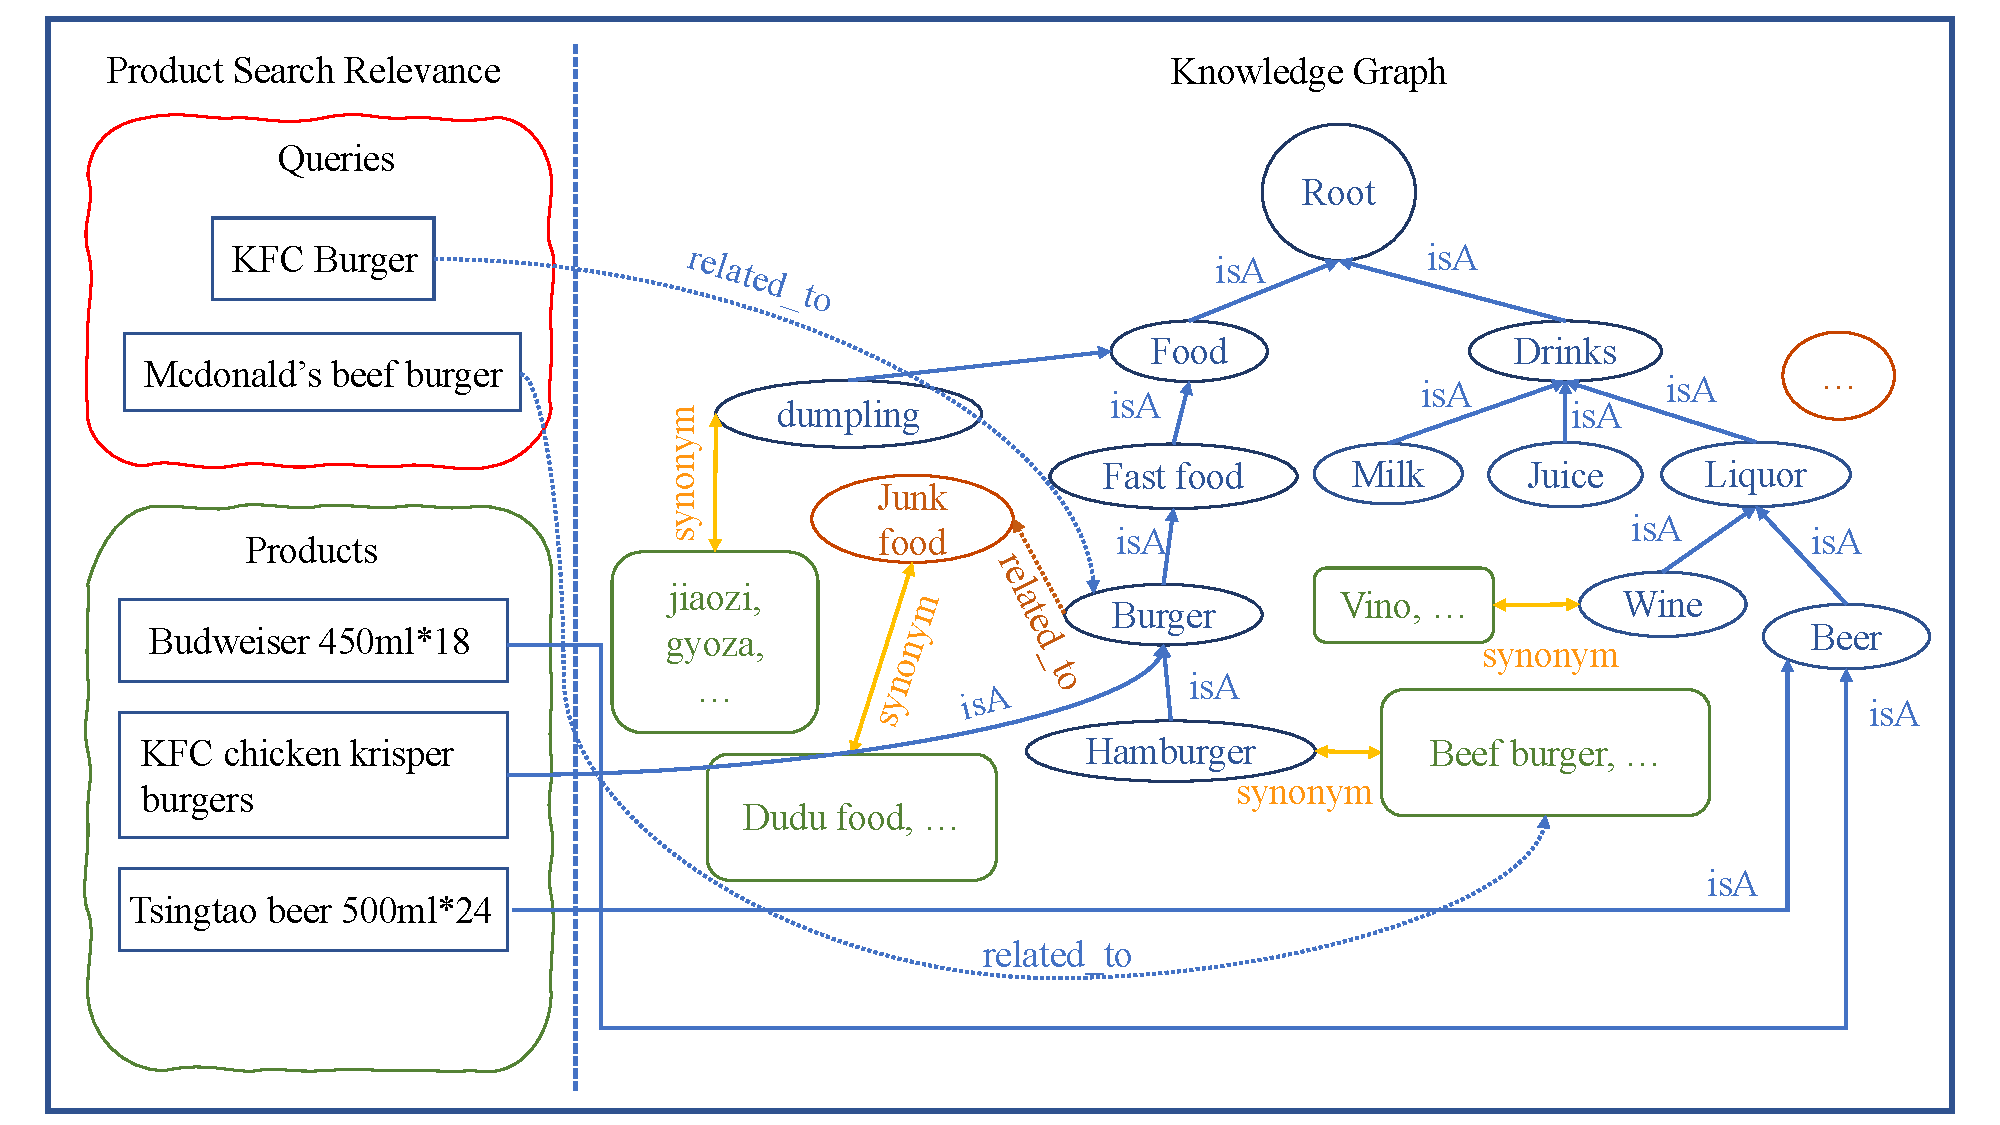
\includegraphics[width=0.99\textwidth]{task_overview_2}
%     \caption{Overview of \textit{Knowledge Graph based Product Search Relevance (KGPSR) Task}.}
%     \label{fig:taskoverview}
% \end{figure*}

\begin{figure}[th] \centering
    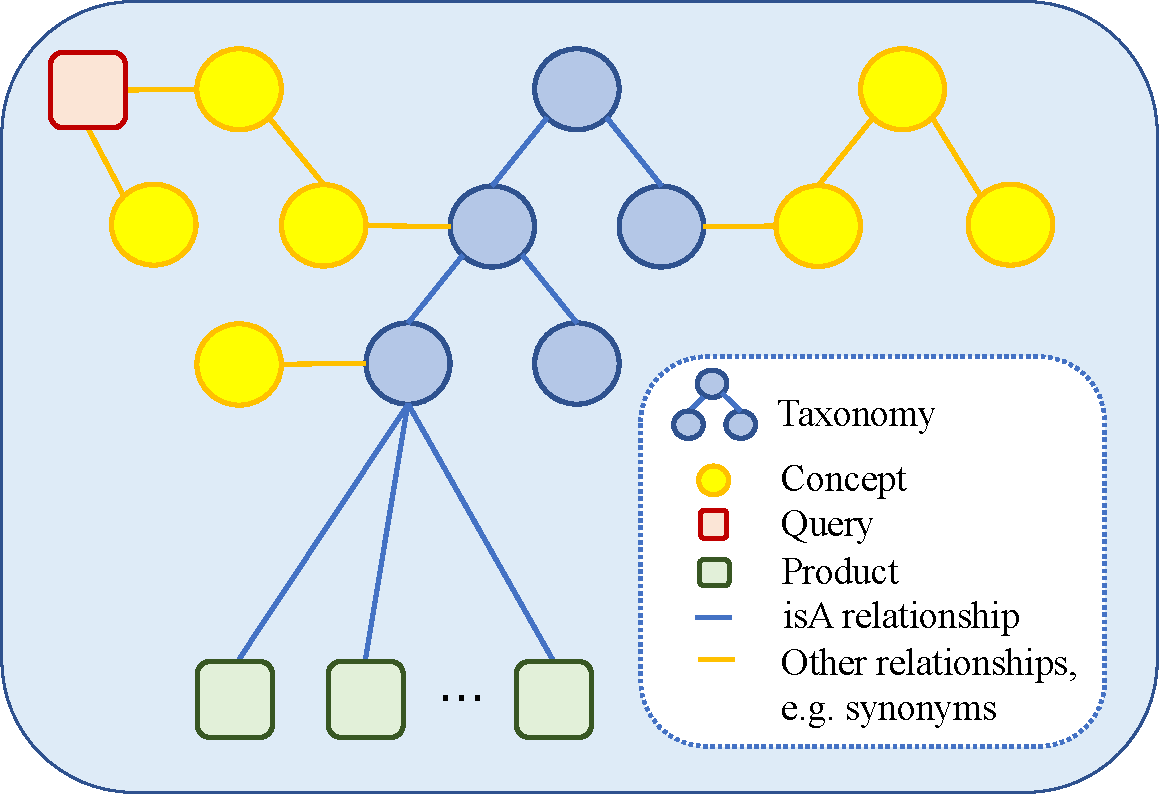
\includegraphics[width=0.4\textwidth]{task_overview3}
    \caption{Overview of Product Search Relevance task with Knowledge Graph. In such task, given a pair of query and product, a PSR model needs to measure the relevance between the query and product with the help of KG.}
    \label{fig:taskoverview}
\end{figure}

% \sansa{\sout{totally unclear about the task. I thought this figure is about the KG structure. You named it TASK, then what is the input and output?}}
% \sansa{\sout{why methods for longer text cannot.} also need citation for the whole paragraph.}

% Currently, due to the short length of both query and product, KG fusion methods can be applied are relatively limited. 

% The most common approaches to fuse KG knowledge into model, such as Knowledge Graph Path (KGP) concatenation \cite{bian2021benchmarking}, Knowledge Graph Embedding (KGE) fusion \cite{luo2021alicoco2}, etc. can only fuse knowledge in a shallow form. 


KG contains a lot of knowledge waiting to be mined and exploited and the knowledge is hidden in relations (e.g. hypernyms, hyponyms, synonyms, etc.), concepts and the KG structure itself. 
In downstream tasks, knowledge is usually utilized in a relatively straightforward and shallow way \cite{bian2021benchmarking, luo2020alicoco, luo2021alicoco2, zhang2021enriching}, such as string concatenation, and embedding fusion, etc. 
These knowledge fusion methods are good at fusing positive relationship knowledge to tell model what an unknown product name or user query is by adding more information such as concepts connected by the query or product in KG.
However, there are still problems that cannot be solved by these methods in our scenario. 
One limitation of these methods is that they have less ability to make use of negative relation knowledge in KG to teach model to distinguish between two vague concepts or products well when positive relationship knowledge is insufficient to handle this problem. 
Note that the positive knowledge represents knowledge relevant to the query or product and negative knowledge represents knowledge less relevant to the query or product. 

For example, for the query product pair ``Green onion'' and ``Seaweed-flavored shallots green onion 65g'' (a kind of snack), even though the positive relation knowledge of the product, ``Snacks / Fried food \& puffed food / Others'', is concatenated to the product name to tell the model the product is not green onion, the similarity score between the query and product is still high. 
This is because ``green onion'' dominates model's understanding of this product and thus model ignores the fused positive relation knowledge or the positive knowledge is ineffective.
We defeine this knowledge fusion problem in PSR task as knowledge ignorance problem and it is usually caused by lexical domination, which means the semantic of query or product is dominated by co-occurring words.

% This problem is more significant in our scenario as query and product name are usually short.
% Our claim is that negative relation knowledge between concepts or products in KG need to be further mined.


% \zelin{sentence too long, hard to understand}
% However, knowledge in KG cannot be deeply mined and utilized by these methods. 

% \zelin{any evidence supporting this statement?}

% \zelin{we'd better explain what is `lexical domination' and cite some works encountering `lexical domination'?}

% Specifically, correct knowledge can be ignored by model with current fusion approach sometimes. 



% In our application scenario, there are still problems cannot be solved by these methods and these problems are mainly caused by \textbf{Underutilized Knowledge Challenge}. 



% However, current methods mainly focus on fuse knowledge by string or embedding concatenation and cannot help model understand the relationship between current query/product and other entities/concepts in KG fundamentally. 

% mine knowledge from KG. 

% In KG construction, products are usually linked to KG by human efforts or models, and both methods will inevitably introduce noise. For instance, product ``Beer Partner 180g/bag'' (a kind of snack) can be mis-linked on the path of ``Snacks - cakes and pastries - bread'' in KG taxonomy. Apperantly, fusing such kind of noisy knowledge in a direct manner does harm to model performance easily. Even though, sometimes knowledge is correct, fusing irrelevant knowledge directly can also cause semantic drift, and this kind of knowledge is also another form of noise. We define this challenge as \textbf{Noisy Knowledge Challenge} in this paper. 

% First, from the perspective of query side, query is usually shorter and contains less information. 

% One critical limitation of conventional knowledge fusion methods 



% This problem is defined as Knowledge Ignorance problem. \sansa{you define a challenge, and then a problem, a little bit weird}

% \sansa{\sout{You just list one problem?}}
% \zelin{... optimize the alignment and uniformity of product text embeddings}
In order to solve the problem mentioned above, negative relation knowledge is necessary to be further utilized to help model understand what the query or product is and is not. 
Thus, we design a novel KG fusion method with contrastive learning called Knowledge Graph \textbf{Con}trastive \textbf{Fu}sion (ConFu) to utilize different kinds of relation knowledge in KG better. 
Our core idea is that by constructing positive and negative samples for query and product based on KG relations, PSR model can learn better embedding containing category or relation knowledge of query and products, so that queries with similar meaning and products with similar categories can be embedded into similar regions in semantic space.
% relations among query/product and other concepts or entities in KG through contrastive learning task to understand user intent and product essence. 
Specifically, with query-side contrastive learning, ConFu can learn knowledge like synonyms and hypernyms of query and learn to distinguish irrelevant queries. 
With product-side contrastive learning, ConFu can learn relations among different products and have a stronger ability to distinguish ambiguous products. 
For the case we mentioned above, ConFu can solve the problem using contrastive learning by embedding the query ``green onion'' and the product into different regions in semantic space.
Another advantage of ConFu is that it does not need external knowledge any more during inference stage. 

Generally speaking, our key contributions are summarized as follows: 

\begin{itemize}
    \item \textbf{A KG based PSR Dataset}. In this paper, we release a novel PSR dataset with KG in life-service e-commerce scenario to call for better solutions. As far as we know, we are the first to release such a Chinese PSR data set with KG. 
    \item \textbf{A Novel KG Fusion Method}. We propose a novel fusion method to inject knowledge in KG into PSR model. With query-side contrastive fusion and product-side contrastive fusion, both positive and negative knowledge in KG can be effectively fused into model to help model understand user need and product names.
    \item \textbf{Effectiveness}. According to our experiments, ConFu can successfully fuse KG into PSR model and benefits PSR task. ConFu outperforms all other baseline methods on KGPSR task by more than 2 points on AUC score. Visualization and case study also demonstrate the effectiveness of ConFu. 
\end{itemize}

% \sansa{\sout{list some specific numbers}}

% \sansa{\sout{Too much space for motivations but no space for methods. Just one sentence for methods?}}
%  With contrastive learning, both positive relationship knowledge and negative relationship knowledge can be injected into model.